%! TEX root = ../main.tex

\titre{Images et matrices de pixels}

\section*{Cheat sheet \texttt{numpy}}

\inputminted{python}{minted/10/cheat_sheet_numpy.py}

\section*{Images en noir et blanc}

\subsection*{Qu'est-ce qu'une image}

\paragraph*{} Une image en noir et blanc en informatique est tout simplement une grille de pixels gris. Un pixel gris contient une unique valeur entre $ 0 $ (noir) et $ 255 $ (blanc) (voir \autoref{fig:grid-of-pixel}). Par exemple, un pixel de valeur $ 50 $ sera gris foncé, et un pixel de valeur $ 200 $ sera gris très clair.

\begin{figure}[h!]
    \begin{center}
        \subfloat[une image grise]{
            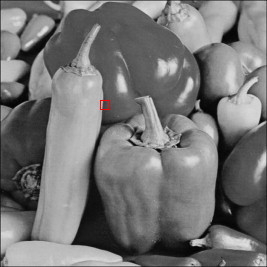
\includegraphics[width=0.45\textwidth]{figures/10/poivrons_grey.png}
        }
        \subfloat[zoom sur le carré rouge]{
            
\includegraphics[width=0.45\textwidth]{figures/10/poivrons_window_grey.png}
        }
    \end{center}
    \caption{Une image est une grille de pixels}
    \label{fig:grid-of-pixel}
\end{figure}

Une image est donc naturellement représentée par une matrice $ M $ d'entiers entre $ 0 $ et $ 255 $. Nous allons utiliser les matrices de \texttt{numpy} pour représenter et manipuler les images. En python, le coin en haut à gauche de l'image correspond au coefficient \texttt{M[0, 0]} de la matrice, comme en mathématiques. Mais attention, comme en mathématiques, le premier indice correspond à l'axe des $ y $ et le second à l'axe des $ x $. On essaye de toujours avoir \autoref{fig:convention-image} en tête. Moyen mnémotechnique : les pixels sont organisés comme lorsqu'on \mintinline{python}{print(M)}.

\begin{figure}[h!]
    \begin{center}
        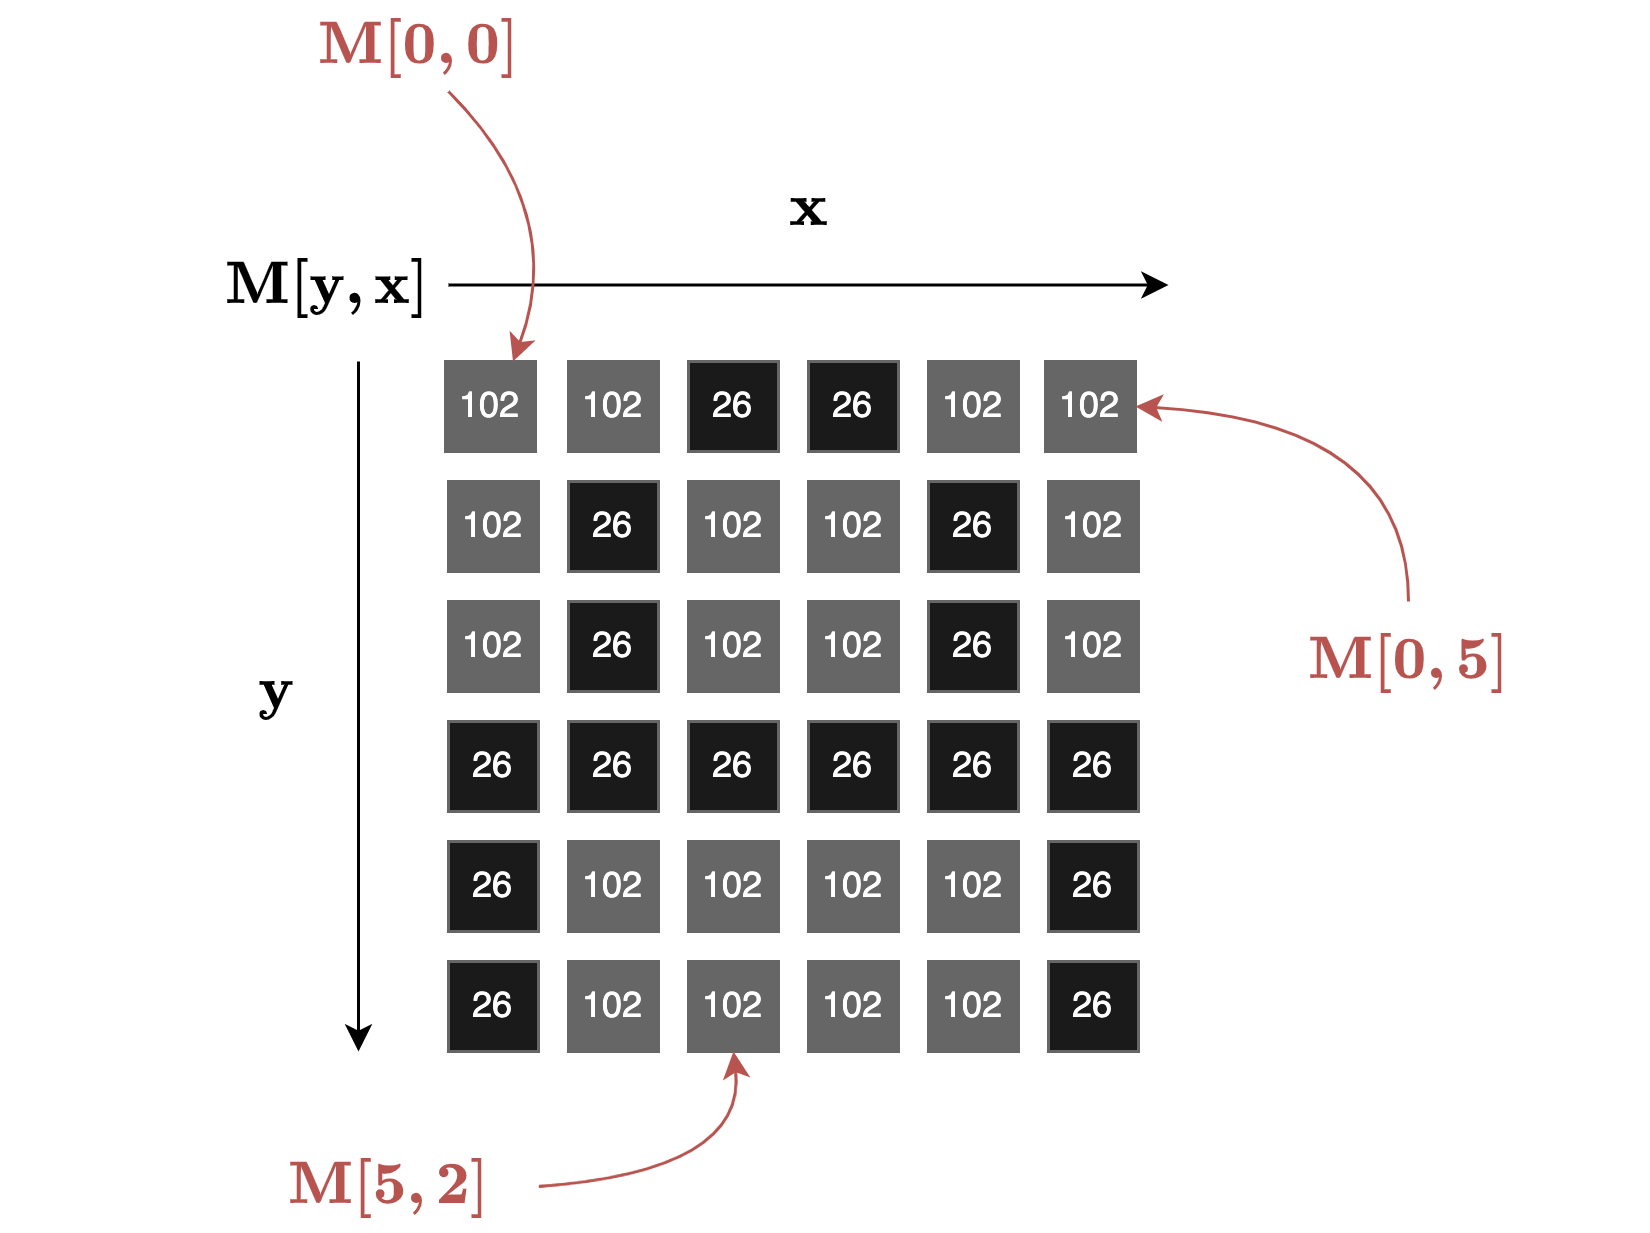
\includegraphics[width=0.65\textwidth]{figures/10/image_grise.png}
    \end{center}
    \caption{ Convention image}
    \label{fig:convention-image}
\end{figure}

\subsection*{Importer, affichage, manipuler, sauver}

\paragraph*{Modules utiles} On utilise le module \texttt{PIL} pour ouvrir, sauvegarder et afficher des images. On utile \texttt{numpy} pour les manipuler.

Écrire dans la console de \texttt{pyzo}
\begin{verbatim}
    pip install Pillow
\end{verbatim}

Puis on écrit en début de fichier 
\begin{minted}{python}
    from PIL import Image
    import numpy as np
\end{minted}

\paragraph*{Importer une image} Téléchargez l'image à l'adresse \href{https://cutt.ly/T4j2eT6}{https://cutt.ly/T4j2eT6} et enregistrez là dans le même dossier que votre fichier python de travail, au nom \texttt{poivrons.png}. Vous pouvez aussi utiliser vos propres images si vous le souhaitez. On peut l'importer dans python avec
\begin{minted}{python}
    img = Image.open('poivrons.png')
\end{minted}

\paragraph*{Afficher une image} On une utilise la méthode \texttt{show()}:
\begin{minted}{python}
    img.show()
\end{minted}

\paragraph*{Obtenir la valeur des pixels sous la forme d'un tableau \texttt{numpy}} Il faut convertir l'image en tableau numpy \emph{et le copier}, sinon on ne peut pas modifier les pixels.
\begin{minted}{python}
    img_grey = img.convert('L') # conversion en image grise
    arr = np.asarray(img_grey).copy()
\end{minted}

\paragraph*{Repasser d'un tableau \texttt{numpy} à une \texttt{Image}}
\begin{minted}{python}
    img = Image.fromarray(arr)
\end{minted}

\paragraph*{sauvegarder une \texttt{Image}}
\begin{minted}{python}
    img.save('poivrons_gris.png', format='PNG')
\end{minted}

\ques Vérifiez que vous arrivez à exécuter les étapes ci-dessus pour finalement produire une version grise de l'image \texttt{poivrons.png}.

\subsection*{Manipulation basique d'image}

\ques Créez les images \autoref{fig:basic-manipulation}

\begin{figure}[!h]
    \begin{center}
        \subfloat[Image mirroir]{
            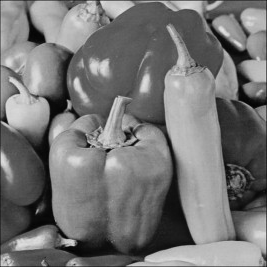
\includegraphics[width=0.3\textwidth]{figures/10/miroir.png}
        }
        \subfloat[Image en négatif]{
            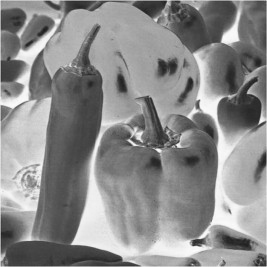
\includegraphics[width=0.3\textwidth]{figures/10/negatif.png}
        }
        \subfloat[Moitié gauche]{
            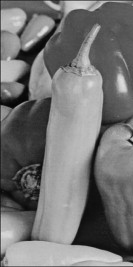
\includegraphics[width=0.15\textwidth]{figures/10/moitie_gauche.png}
        }
    \end{center}
    \caption{Manipulations basiques d'images}
    \label{fig:basic-manipulation}
\end{figure}

\subsection*{Jeu sur la luminosité}

Le but de cette question est d'éclaircir une image. Pour éclaircir une image, il faut globalement augmenter la valeur des pixels. Mais attention, on ne peut pas juste ajouter une constante car la valeur des pixels ne doit pas dépasser 255. À la place, il faut trouver une fonction \[
    eclair:
    \begin{cases}
        [0, 255] &\rightarrow [0, 255]\\
        pixel &\mapsto \quad ?
    \end{cases}
\]
telle que $ eclair(x) \geq x $.

\quessques Donner une fonction qui ressemble à celle \autoref{fig:eclair-func}

\begin{figure}[h!]
    \begin{center}
        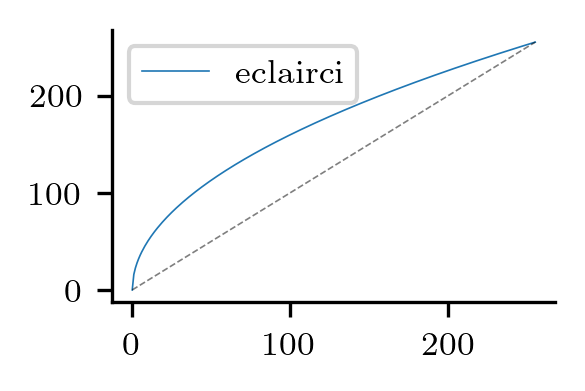
\includegraphics[width=0.4\textwidth]{figures/10/eclair_func.png}
    \end{center}
    \caption{Fonction d'éclaircissement}
    \label{fig:eclair-func}
\end{figure}

\ssques Appliquer la fonction à chaque pixel de l'image et vérifier qu'on obtient une image éclaircie, similaire à \autoref{fig:img-eclaircie}. Attention, par défaut lorsqu'on lit une \texttt{Image} dans un tableau \texttt{numpy}, les valeurs sont de type \texttt{np.uint8}, c'est à dire des entiers de $ [\![0, 255]\!] $ et les calculs se font alors dans $ \Z / 256 \Z $. Pour sortir de ce mode de calcul, il faut faire une conversion explicite vers \texttt{np.float64} en début de calcul, puis reconvertir en \texttt{np.uint8} à la fin des calculs.

\begin{minted}{python}
    arr = arr.astype(np.float64)
    ... # opérations sur arr
    arr = arr.astype(np.uint8)
\end{minted}

\begin{figure}[h!]
    \begin{center}
        \subfloat[Image éclaircie]{
            \label{fig:img-eclaircie}
            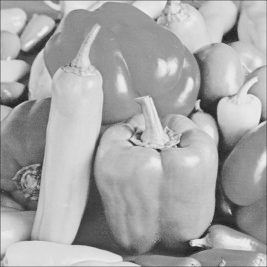
\includegraphics[width=0.4\textwidth]{figures/10/eclairci.png}
        }
        \subfloat[Image assombrie]{
            \label{fig:img-assombrie}
            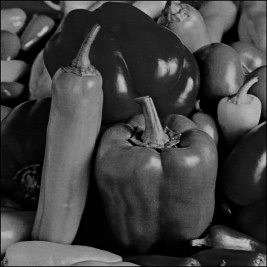
\includegraphics[width=0.4\textwidth]{figures/10/noirci.png}
        }
    \end{center}
    \caption{Changement de luminosité}
\end{figure}

\ssques Trouver une transformation pour obtenir une image cette fois-ci assombrie, comme \autoref{fig:img-assombrie}.

\subsection*{Jeu sur les contrastes}

Une image est très contrastée lorsque les zones sombres sont très sombres et les zones claires très claires, c'est-à-dire que l'ensemble des valeurs des pixels a une grande variance. À l'inverse, une image est peu contrastée si elle est globalement grise, c'est-à-dire que l'ensemble des valeurs des pixels a une faible variance. 


\quessques Trouver deux fonctions dont le graphe ressemble à ceux \autoref{fig:contraste-funcs}

\begin{figure}[h!]
    \begin{center}
        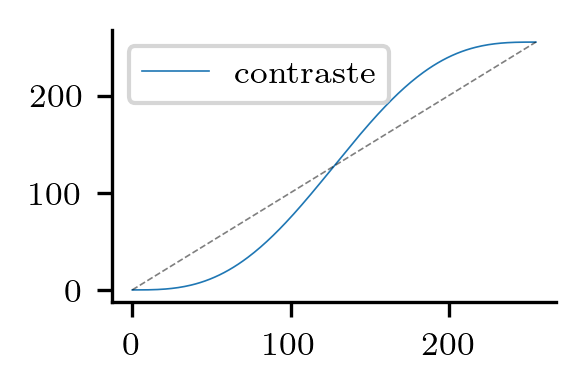
\includegraphics[width=0.4\textwidth]{figures/10/contraste_func.png}
        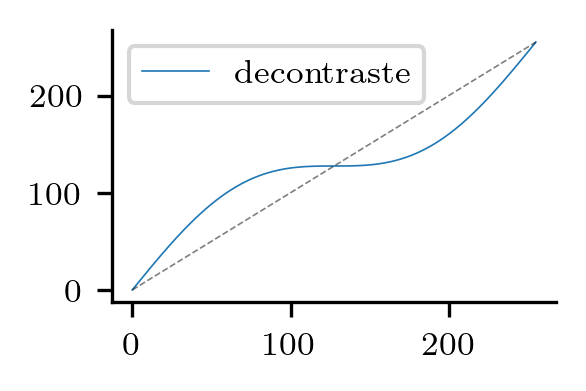
\includegraphics[width=0.4\textwidth]{figures/10/decontraste_func.png}
    \end{center}
    \caption{Fonctions de contrastes}
    \label{fig:contraste-funcs}
\end{figure}

\ssques Recréer les images \autoref{fig:contraste-imgs}

\begin{figure}[h!]
    \begin{center}
        \subfloat[Image contrastée]{
            \label{fig:img-contrast}
            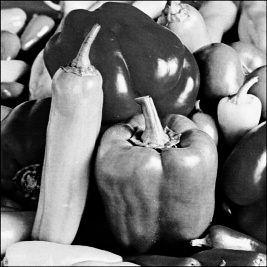
\includegraphics[width=0.4\textwidth]{figures/10/contraste.png}
        }
        \subfloat[Image peu contrastée]{
            \label{fig:img-low-contrast}
            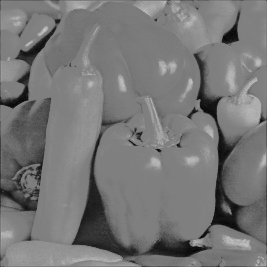
\includegraphics[width=0.4\textwidth]{figures/10/decontraste.png}
        }
    \end{center}
    \caption{Changement de contrastes}
    \label{fig:contraste-imgs}
\end{figure}


% \section*{Représenter la couleur}
% \paragraph*{Qu'est-ce qu'une image en informatique ?} En informatique, une image est un ensemble structuré de pixels. On représente une image par une matrice contenant la valeur de chacun de ses pixels. Traditionnellement, un pixel est un triplet de valeur $ (r, g, b) $ représentant la quantité de rouge $ r $, la quantité de vert $ g $ et la quantité de bleu $ b $. D'ailleurs si vous prenez une loupe et zoomez sur votre écran (d'ordinateur ou de téléphone), vous pourrez voir apparaître des diodes individuelles rouges, vertes et bleues. Ce phénomène peut aussi avoir lieu en déposant une goutte d'eau sur l'écran.
